%package list
\documentclass{article}
\usepackage[top=3cm, bottom=3cm, outer=3cm, inner=3cm]{geometry}
\usepackage{graphicx}
\usepackage{url}

%% \usepackage{cite}
\usepackage{hyperref}
\usepackage{array}
\usepackage{multicol}
\newcolumntype{x}[1]{>{\centering\arraybackslash\hspace{0pt}}p{#1}}
\usepackage{natbib}
\usepackage{pdfpages}
\usepackage{multirow}
\usepackage{float}
\usepackage[normalem]{ulem}
\useunder{\uline}{\ul}{}


%%%%%%%%%%%%%%%%%%%%%%%%%%%%%%%%%%%%%%%%%%%%%%%%%%%%%%%%%%%%%%%%%%%%%%%%%%%%
%%%%%%%%%%%%%%%%%%%%%%%%%%%%%%%%%%%%%%%%%%%%%%%%%%%%%%%%%%%%%%%%%%%%%%%%%%%%
\newcommand{\csemail}{vmachacaa@unsa.edu.pe}
\newcommand{\csdocente}{Vicente Machaca Arceda}
\newcommand{\cscurso}{Algoritmos y Estructura de Datos}
\newcommand{\csuniversidad}{Universidad Nacional de San Agustín}
\newcommand{\csescuela}{Maestría en Ciencia de la Computación}
\newcommand{\cspracnr}{04}
\newcommand{\cstema}{--}
%%%%%%%%%%%%%%%%%%%%%%%%%%%%%%%%%%%%%%%%%%%%%%%%%%%%%%%%%%%%%%%%%%%%%%%%%%%%
%%%%%%%%%%%%%%%%%%%%%%%%%%%%%%%%%%%%%%%%%%%%%%%%%%%%%%%%%%%%%%%%%%%%%%%%%%%%


\usepackage[english,spanish]{babel}
\usepackage[utf8]{inputenc}
\AtBeginDocument{\selectlanguage{spanish}}
\renewcommand{\figurename}{Figura}
\renewcommand{\refname}{Referencias}
\renewcommand{\tablename}{Tabla} %esto no funciona cuando se usa babel
\AtBeginDocument{%
	\renewcommand\tablename{Tabla}
}

\usepackage{fancyhdr}
\pagestyle{fancy}
\fancyhf{}
\setlength{\headheight}{30pt}
\renewcommand{\headrulewidth}{1pt}
\renewcommand{\footrulewidth}{1pt}
\fancyhead[L]{\raisebox{-0.2\height}{
\includegraphics[width=3cm]{img/logo_unsa.jpg}}}
\fancyhead[C]{}
\fancyhead[R]{\fontsize{7}{7}\selectfont	\csuniversidad \\ \csescuela \\ \textbf{\cscurso} }
\fancyfoot[L]{MSc. Vicente Machaca}
\fancyfoot[C]{\cscurso}
\fancyfoot[R]{Página \thepage}

\begin{document}
	
	\vspace*{10px}
	
	\begin{center}	
		\fontsize{17}{17} \textbf{ Práctica \cspracnr}
	\end{center}
	%\centerline{\textbf{\underline{\Large Título: Informe de revisión del estado del arte}}}
	%\vspace*{0.5cm}
	

	\begin{table}[h]
		\begin{tabular}{|x{4.7cm}|x{4.8cm}|x{4.8cm}|}
			\hline 
			\textbf{DOCENTE} & \textbf{CARRERA}  & \textbf{CURSO}   \\
			\hline 
			\csdocente & \csescuela & \cscurso    \\
			\hline 
		\end{tabular}
	\end{table}	
	
	
	\begin{table}[h]
		\begin{tabular}{|x{4.7cm}|x{4.8cm}|x{4.8cm}|}
			\hline 
			\textbf{PRÁCTICA} & \textbf{TEMA}  & \textbf{DURACIÓN}   \\
			\hline 
			\cspracnr & Proyecto Final & 3 horas   \\
			\hline 
		\end{tabular}
	\end{table}
	
	
	\section{Datos de los estudiantes}
	\begin{itemize}
		\item Grupo: V
		\item Integrantes: 
		\begin{itemize}
			\item Angel Yvan Choquehuanca Peraltilla
			\item Estefany Pilar Huaman Colque
            \item Eduardo Diaz Huayhuas
            \item Gustavo Raul Manrique Fernandez
		\end{itemize}		
	\end{itemize}
	
	
 
	
	%\clearpage
	%\bibliographystyle{apalike}
	%\bibliographystyle{IEEEtranN}
	%\bibliography{bibliography}
		

\section{Introducción}
   Actualmente, el aumento y la  digitalización de los hospitales, especialmente en el diagnóstico  por imagen, y la necesidad de comunicaciones médicas, ha puesto de relieve la necesidad de estandarizar los protocolos de comunicación y los formatos de la información en sanidad. 
   Uno de los estándares más exitosos hasta la fecha es DICOM (Digital Imaging and Communications in Medicine). 
   
   Para la detección de patologias como el COVID-19, se utiliza algoritmos avanzados para la detección de estas anomalías. 
   
    En este proyecto final, utilizaremos un algoritmo que permita detectar estas anomalias a partir de imagenes DICOM y con ello generar diagnosticos preliminares con el fin de acelerar la atención hospitalaria.

    
\section{Marco Teorico}
\subsection{Que es DICOM}

\begin{figure}[H]
\centering

\includegraphics[width=0.7\textwidth]{img/dicom.jpg}
\caption{DICOM}
\end{figure}


DICOM es un protocolo estándar de comunicación entre sistemas de información y a la vez un formato de almacenamiento de imágenes médicas que aparece como solución a los problemas de interoperabilidad entre tipos de dispositivos.

Una imagen médica por sí misma no aporta suficiente información. Para que sea correctamente interpretada es necesario que vaya acompañada de datos del paciente y de la adquisición. Por eso formatos tradicionales como él .jpeg o el .png se quedan cortos.

\subsection{Caracteristicas del Formato DICOM}
El formato DICOM cuenta con objetos IOD (Information Object Definition), formados por la imagen y su información asociada (Son una representación lógica de objetos del mundo real) y DIMSE (DICOM Message Service Element), operaciones que pueden realizarse sobre un objeto. IOD y DICOM forman SOP, la unidad funcional de DICOM.

Un IOD se compone de IEs (Entidades de información) (Hay IE de paciente, de estudio, de serie,  de equipo, de imagen…) que a su vez se componen de uno o varios módulos que a su vez se contienen varios atributos. Un atributo se define con nombre, etiqueta, tipo y descripción.

\subsection{Composición del estandar DICOM}

\begin{figure}[H]
\centering
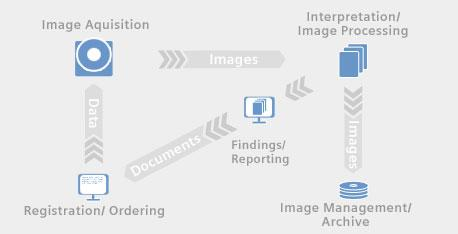
\includegraphics[width=0.7\textwidth]{img/dicom_diagram.jpg}
\caption{Diagrama del proceso para el analisis de imagenes DICOM}
\end{figure}

En el estándar DICOM la información se define mediante un modelo que refleja el mundo real. La imagen es el núcleo de información de un fichero DICOM. Cada fichero contiene, además de la imagen, información sobre el paciente (identificación demográfica y de identificación), el estudio en el que se encuadra la toma de la imagen, la serie a la que pertenece la imagen e información sobre la propia imagen.

\subsection{Importancia del estandar DICOM}

\begin{figure}[H]
\centering
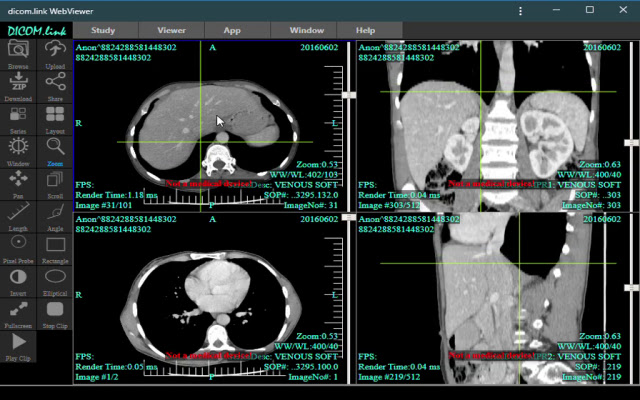
\includegraphics[width=0.7\textwidth]{img/dicom_real.jpg}
\caption{Uso de Software para analisar patologias o anomalias usando DICOM}
\end{figure}

DICOM permite una identificación univoca de objetos. Cada fichero DICOM tiene un UID único compuesto por varios números.

Las comunicaciones DICOM se adaptan al estándar OSI para el intercambio de información. La AE (Entidad de Aplicación) se encarga de las comunicaciones de modo que para cada servicio existe un AE cliente y un AE aplicación.

Gracias a sus características y a su nivel de implantación, hoy día DICOM es mundialmente reconocido para el manejo, almacenamiento, impresión y transmisión de imágenes médicas.


\section{Metodologia y Desarrollo}

\subsection{Preparación del entorno de desarrollo}
\subsection{Procesamiento de la Imagen}
\subsection{Utilizando el Algoritmo Quadtree}
\subsection{Output: Detectando las patologias}




\section{Resultados}
\subsection{Imagenes procesadas}



\section{Conclusiones}


	
	
	\end{document}
